\documentclass[11pt,a4paper]{article}
\usepackage[utf8]{inputenc}
\usepackage[spanish]{babel}
\usepackage[T1]{fontenc}
\usepackage[margin=2.5cm]{geometry}
\usepackage{graphicx}
\usepackage{booktabs}
\usepackage{longtable}
\usepackage{array}
\usepackage{float}
\usepackage{xcolor}
\usepackage{hyperref}
\usepackage{enumitem}
\usepackage{titlesec}
\usepackage{parskip}

\titleformat{\section}{\normalfont\Large\bfseries\color{blue!40!black}}{P\thesection.}{0.5em}{}
\titleformat{\subsection}{\normalfont\large\bfseries}{\thesubsection}{0.5em}{}

\hypersetup{colorlinks=true, linkcolor=blue, urlcolor=blue}

\title{\textbf{Prueba Pr\'actica -- Unidad IV \\ Ingenier\'ia de Requisitos (ISR-401) \\ Caso: Sistema de Gesti\'on de Pedidos}}
\author{Erick Jahir Quintero Gende \\ 4to Software ``A''}
\date{\today}

\begin{document}
\maketitle

\begin{center}

\end{center}

\vspace{0.5cm}
\noindent\textbf{Descripci\'on del caso.} Una tienda en l\'inea requiere un m\'odulo para gestionar los pedidos de sus clientes. Un \textbf{Cliente} (identificado por c\'edula/RUC, nombre y correo) puede realizar cero o m\'as \textbf{Pedidos}. Cada \textbf{Pedido} (identificador, fecha y total) contiene una o m\'as \textbf{L\'ineas de pedido}, y cada l\'inea referencia un \textbf{Producto} (c\'odigo, descripci\'on, precio, stock). Al registrar un pedido, el sistema verifica la disponibilidad de stock: si hay existencias, confirma el pedido; si no, notifica el faltante. Un pedido confirmado puede despacharse, luego entregarse, o bien anularse mientras no haya sido entregado.

\section{Modelo de datos -- Diagrama de clases UML}


\begin{figure}[h]
\centering
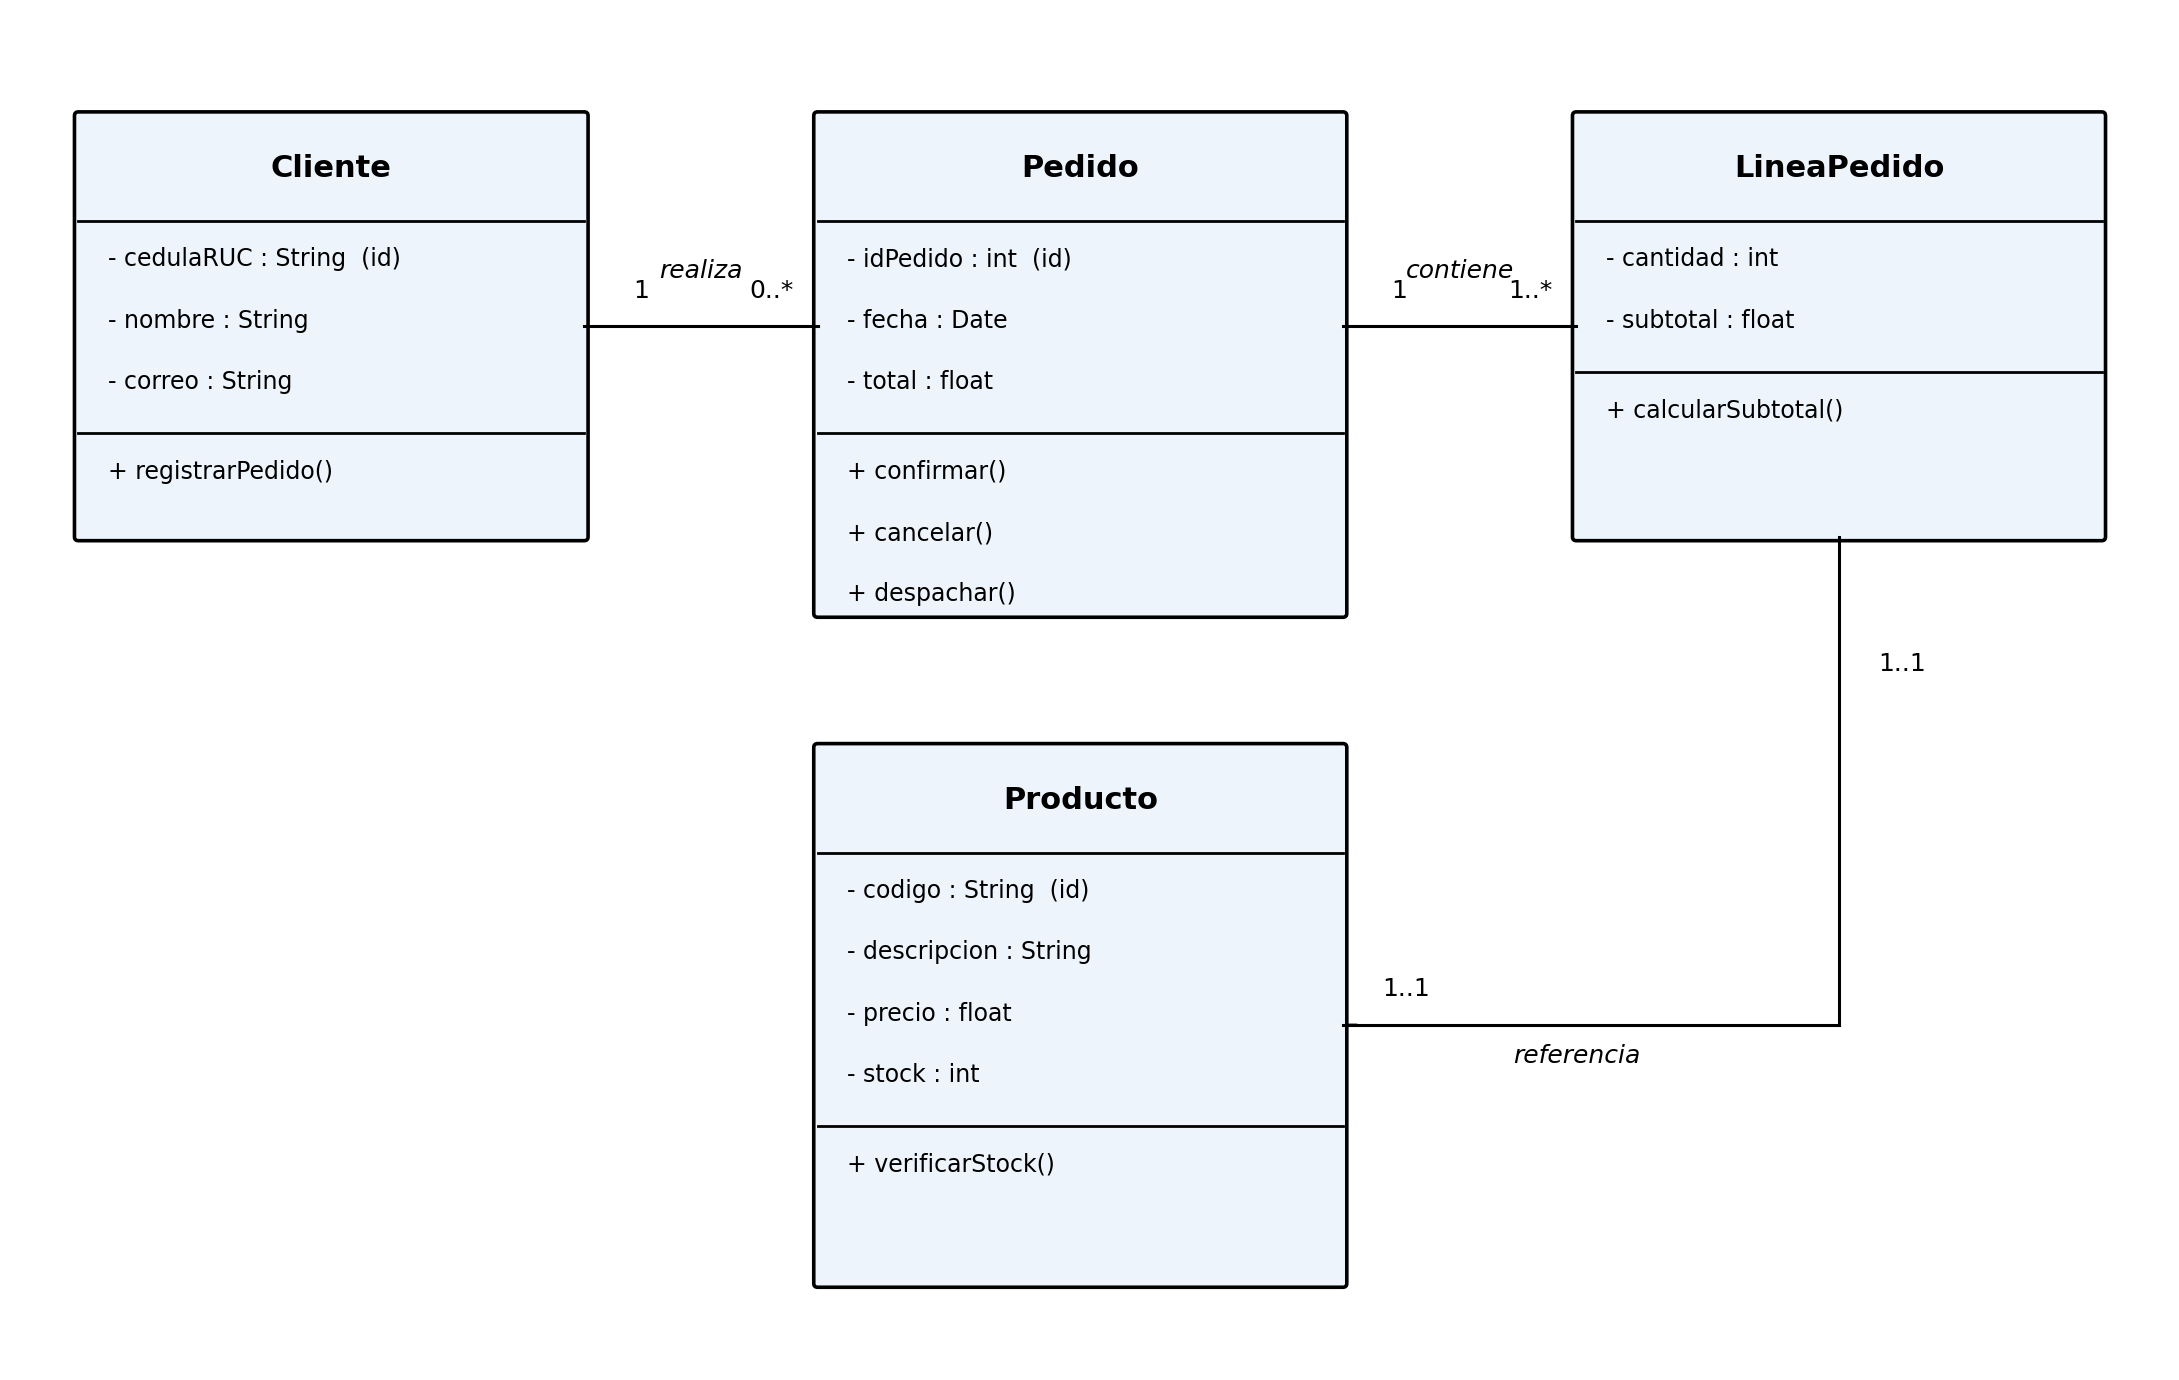
\includegraphics[width=0.95\textwidth]{figuras/p1_diagrama_clases.png}
\label{fig:clases}
\end{figure}



\section{Modelo funcional -- Diagrama de actividades UML}

\begin{figure}[h]
\centering
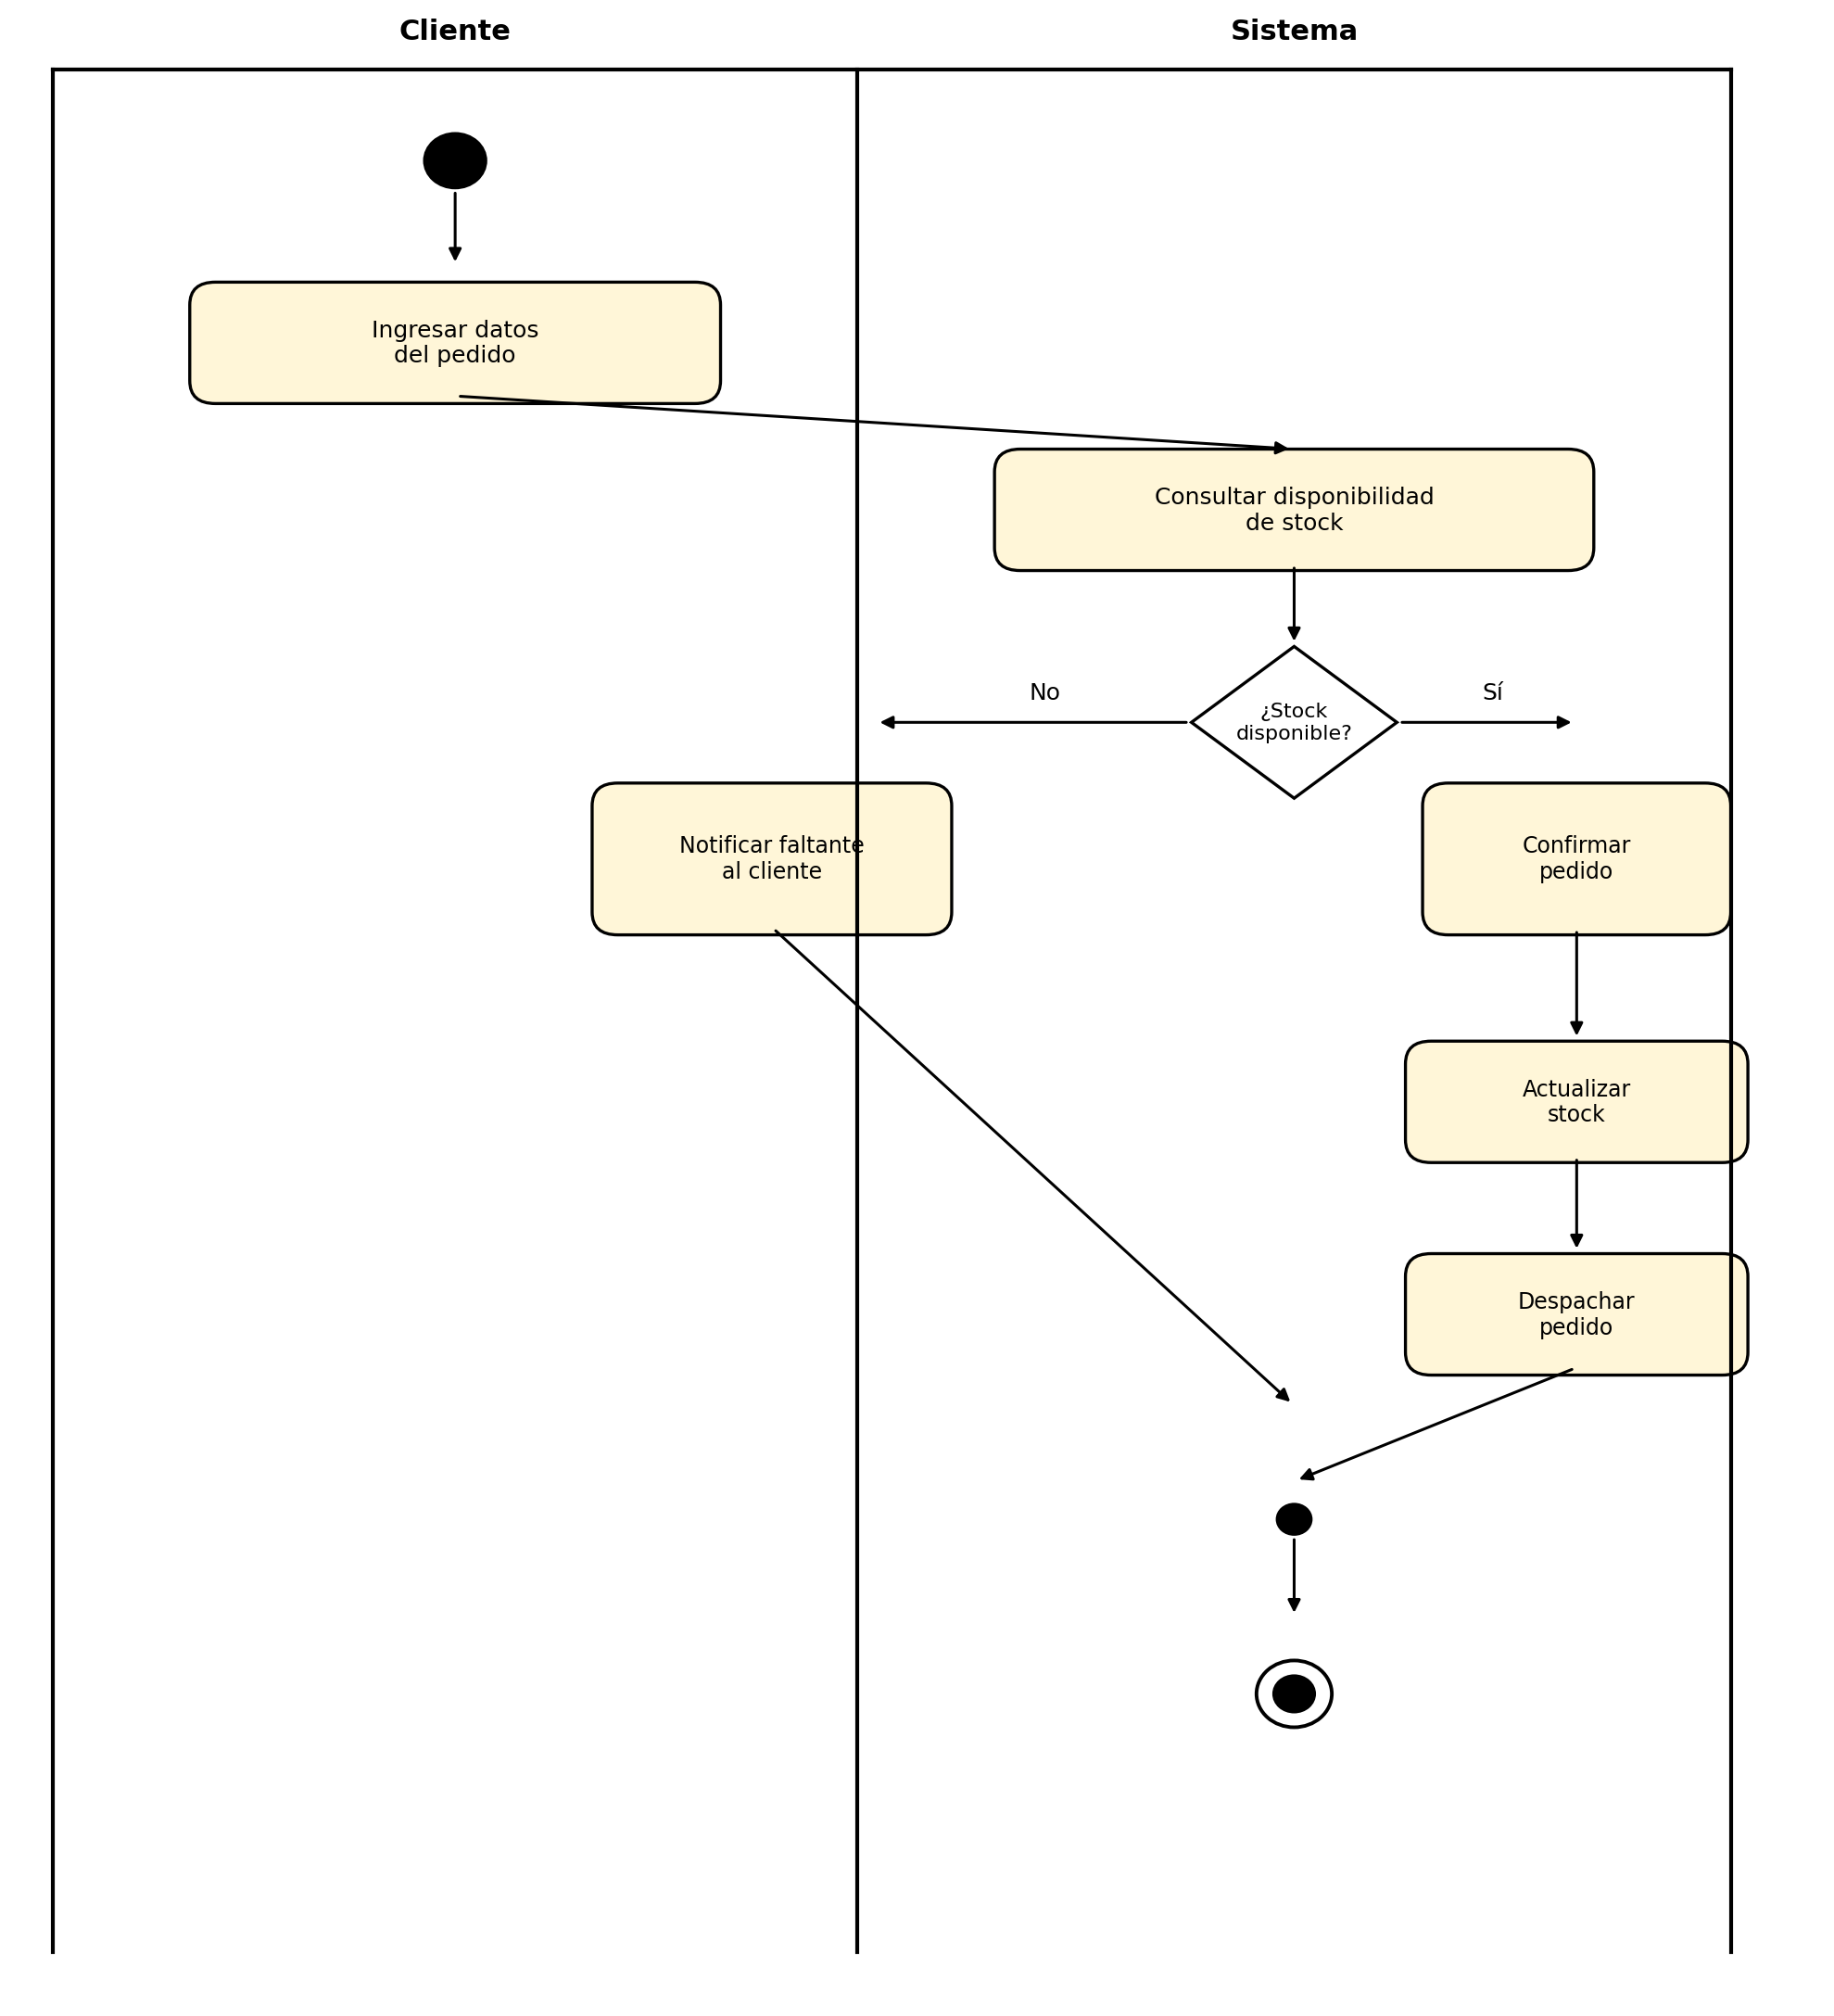
\includegraphics[width=0.85\textwidth]{figuras/p2_diagrama_actividades.png}
\label{fig:actividades}
\end{figure}



\section{Modelo de comportamiento -- M\'aquina de estados UML}

\begin{figure}[H]
\centering
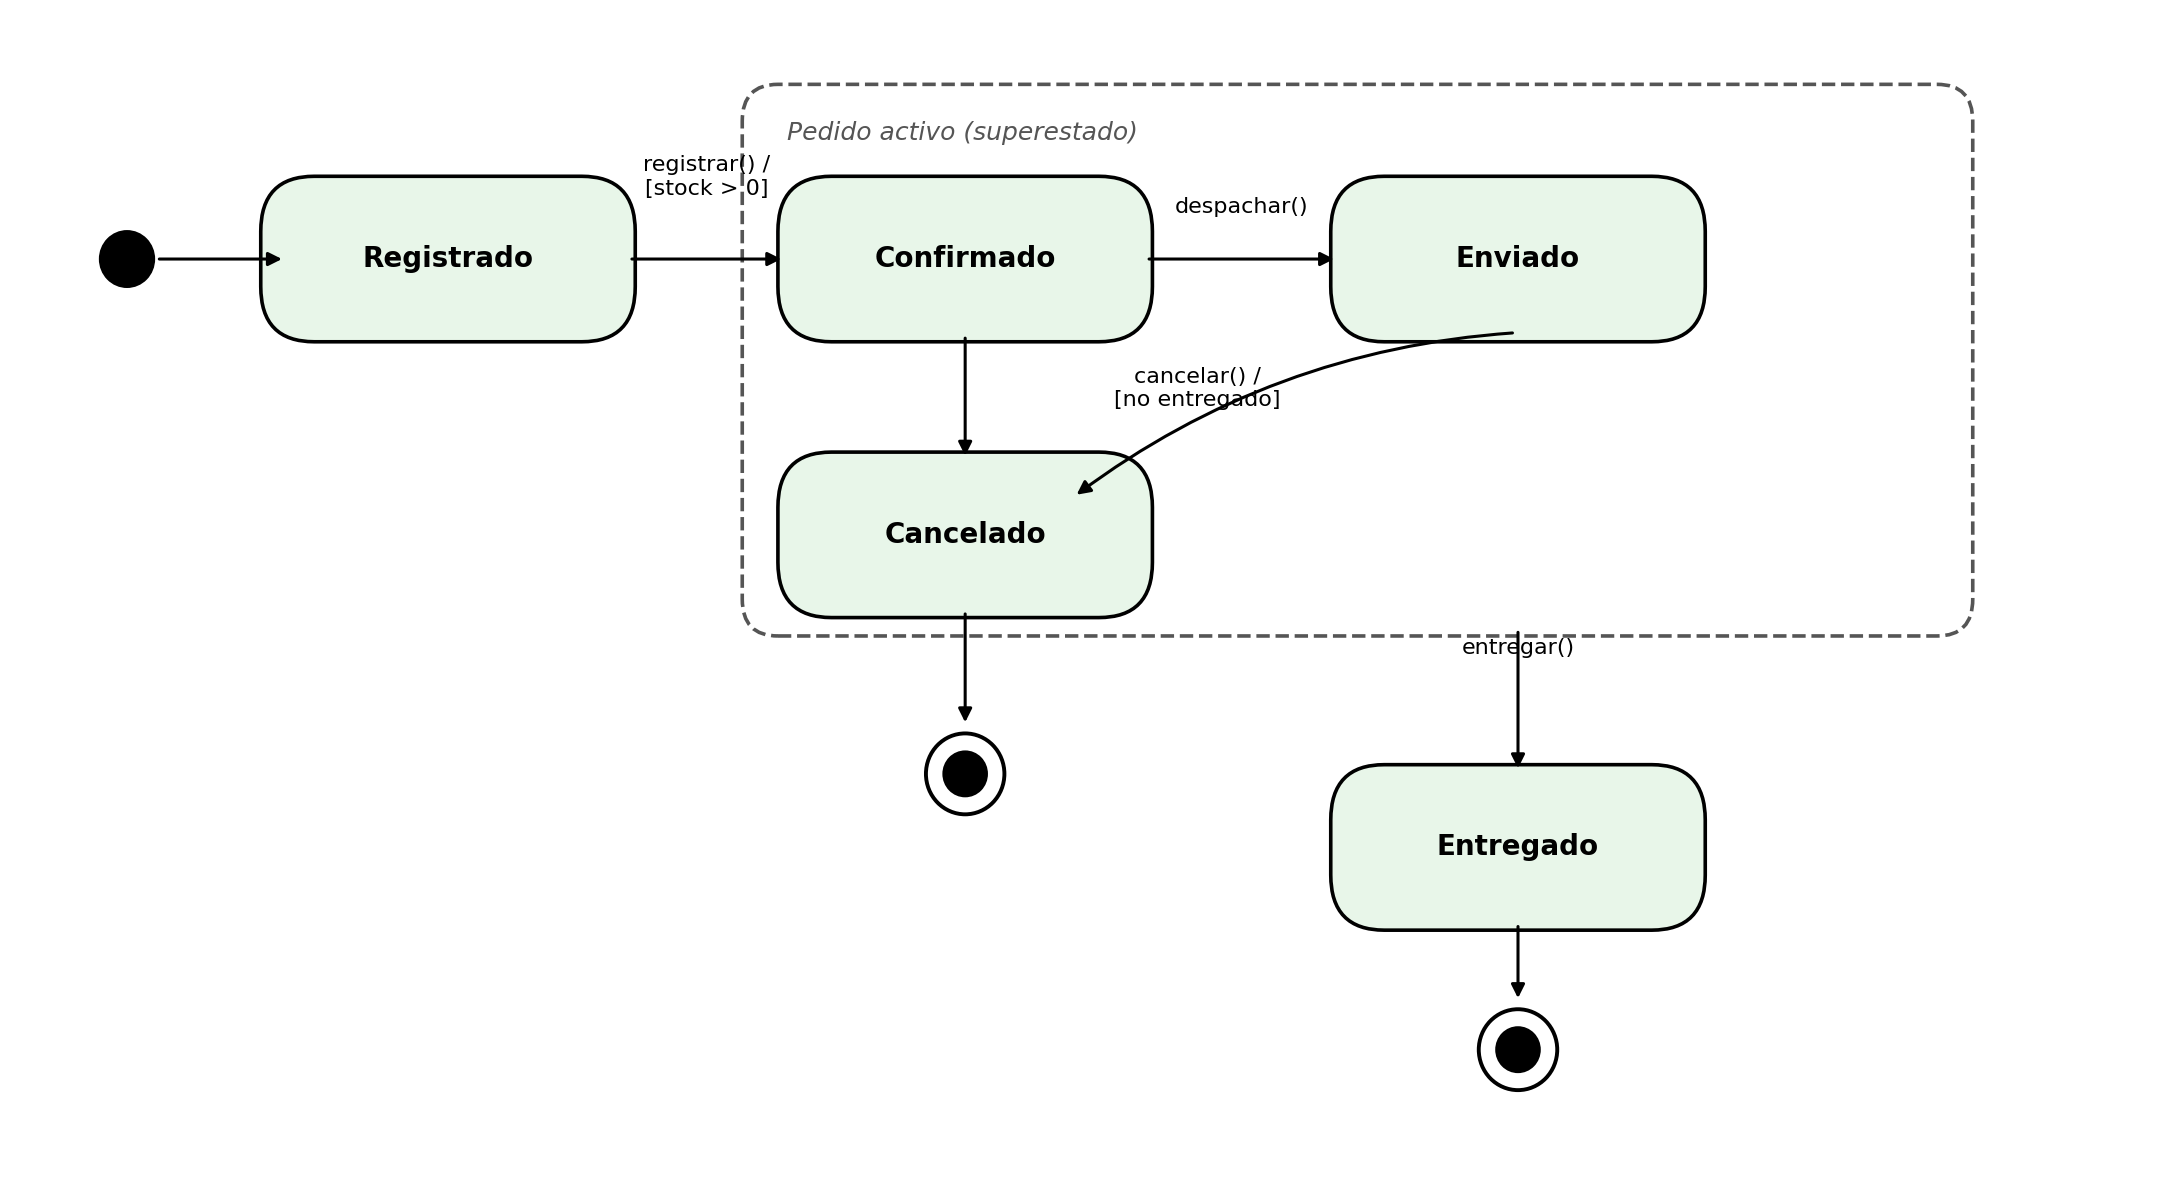
\includegraphics[width=0.95\textwidth]{figuras/p3_maquina_estados.png}
\caption{M\'aquina de estados UML del ciclo de vida de un Pedido.}
\label{fig:estados}
\end{figure}

\section{Consistencia entre las tres perspectivas}


\begin{table}[h]
\centering
\begin{tabular}{lll}
\toprule
\textbf{Evento (P3)} & \textbf{Funci\'on/Actividad (P2)} & \textbf{Entidad/Atributo (P1)} \\
\midrule
registrar() & Ingresar datos del pedido & Pedido.idPedido \\

confirmar() & Confirmar pedido & idconfirmar\\

despachar() & Despachar pedido & Pedido.idPedido (estado) \\
cancelar() & Notificar faltante / anulaci\'on & Pedido.total \\
notificar faltante() & notificar faltante & idnotificacion \\
\bottomrule
\end{tabular}

\end{table}



\section{Especificaci\'on de requisitos con esquema de atributos}


\begin{table}[H]
\centering
\small
\begin{tabular}{p{1.7cm}p{6.3cm}p{1.5cm}p{1.4cm}p{1.7cm}p{1cm}p{1cm}p{2.2cm}}
\toprule
\textbf{ID} & \textbf{Descripci\'on} & \textbf{Prioridad} \\
\midrule
RF-01 & El sistema debe registrar un pedido validando la disponibilidad de stock del producto solicitado. & Alta  \\
RF-02 & El sistema debe permitir cancelar un pedido mientras su estado sea Confirmado y no haya sido entregado. & Media \\
RNF-01 & [\emph{Eficiencia de desempe\~no}] El sistema debe registrar un pedido en menos de 3 segundos. & Alta \\
RNF-02 & [\emph{Seguridad}] Los datos personales del cliente deben almacenarse cifrados con AES-256. & Media \\
\bottomrule
\end{tabular}

\end{table}

\section{Priorizaci\'on MoSCoW}

\begin{table}[h]
\centering
\begin{tabular}{lll p{7.5cm}}
\toprule
\textbf{Requisito} & \textbf{Categor\'ia} & & \textbf{Justificaci\'on} \\
\midrule
RF-01 & \textbf{Must have} & & Responde al objetivo central del sistema: sin validaci\'on de stock no existe un registro de pedidos confiable. \\
RF-02 & \textbf{Must have} & & Es importante para la experiencia del cliente, pero el sistema puede operar (con soporte manual) sin esta funci\'on en una primera versi\'on. \\
RNF-01 & \textbf{Should have} & & El tiempo de respuesta es un requisito m\'inimo de aceptaci\'on del negocio (rendimiento cr\'itico). \\
RNF-02 & \textbf{Should have} & & Es una mejora deseable de seguridad, factible de incorporar en una iteraci\'on posterior sin bloquear el lanzamiento. \\
\bottomrule
\end{tabular}
\end{table}


\section{Validaci\'on por inspecci\'on (checklist ISO/IEC/IEEE 29148)}


\begin{table}[h]
\centering
\begin{tabular}{llp{8.5cm}}
\toprule
\textbf{Requisito} & \textbf{Propiedad violada} & \textbf{Defecto detectado} \\
\midrule
RF-02 & No ambiguo & El verbo ``cancelar'' no especifica bajo qu\'e condici\'on de estado es v\'alida la acci\'on. \\
RF-01 & Verificable / Completo & No se especifica el m\'etodo de verificaci\'on del cifrado, por lo que no es comprobable objetivamente. \\
RNF-01 & Singular & Puede ser no verificable \\
RNF-02 & Completo & No de puede ver a simple vista \\
\bottomrule
\end{tabular}

\end{table}


\begin{itemize}[nosep]
    \item \textbf{RF-02 (corregido):} ``El sistema debe permitir cancelar un pedido mientras su estado sea Confirmado y no haya sido entregado.''
    \item \textbf{RNF-02 (corregido):} ``Los datos personales del cliente deben almacenarse cifrados con AES-256, verificado mediante prueba de penetraci\'on.''
\end{itemize}


\section{Pruebas de aceptaci\'on trazadas}

\begin{table}[h]
\centering
\small
\begin{tabular}{lp{1.6cm}p{4.2cm}p{4.5cm}p{1.3cm}}
\toprule
\textbf{Prueba} & \textbf{Tipo} & \textbf{Entradas} & \textbf{Criterio de \'exito} & \textbf{Traza} \\
\midrule
PA-01 & Funcional & Pedido con producto de stock $>0$ & El pedido queda en estado Confirmado & RF-01 \\
PA-02 & Funcional & Pedido en estado Confirmado, no entregado & El estado del pedido cambia a Cancelado & RF-02 \\
PA-03 & No funcional & 100 registros de pedido consecutivos & El 95\% se registra en $<3$\,s & RNF-01 \\
PA-04 & No funcional & Inspecci\'on de la base de datos de clientes & Los campos personales aparecen cifrados con AES-256 & RNF-02 \\
\bottomrule
\end{tabular}

\end{table}

\section{Matriz de trazabilidad}

\begin{table}[h]
\centering
\small
\begin{tabular}{lllll}
\toprule
\textbf{Requisito} & \textbf{Fuente} & \textbf{Modelo (P1--P3)} & \textbf{Prueba (P8)} & \textbf{Dependencia} \\
\midrule
RF-01 & Cliente & P1, P2, P3 & PA-01 & RNF-01 \\
RF-02 & Cliente & P1, P3 & PA-02 & -- \\
RNF-01 & Norma 25010 & P2 & PA-03 & RF-01 \\
RNF-02 & Norma 25010 & P1 & PA-04 & -- \\
\bottomrule
\end{tabular}
\end{table}


\section{Gesti\'on del cambio y l\'inea base}

\subsection*{Solicitud de cambio}
\begin{itemize}[nosep]
    \item \textbf{Solicitante:} Erick Quintero (rol: Inspector)
    \item \textbf{Cambio solicitado:} Modificar RNF-01 para registrar el pedido en menos de 2 segundos (en lugar de 3 segundos).
   
    \item \textbf{Decisi\'on del CCB:} \textbf{Rechazada}, por no ser viable con la infraestructura actual del sistema.
    \item \textbf{Versi\'on actualizada:} RNF-01 v1.1 (se mantiene el umbral de $<3$\,s; se documenta la solicitud rechazada como antecedente).
\end{itemize}

\subsection*{L\'inea base declarada}

\begin{itemize}[nosep]
    \item ERS v1.1 (especificaci\'on de requisitos de P5--P7).
    \item Modelos P1--P3 (diagrama de clases, actividades y m\'aquina de estados).
    \item Matriz de trazabilidad P9.
    \item Conjunto de pruebas de aceptaci\'on P8.
\end{itemize}

\end{document}
